% Options for packages loaded elsewhere
\PassOptionsToPackage{unicode}{hyperref}
\PassOptionsToPackage{hyphens}{url}
%
\documentclass[
]{article}
\usepackage{amsmath,amssymb}
\usepackage{iftex}
\ifPDFTeX
  \usepackage[T1]{fontenc}
  \usepackage[utf8]{inputenc}
  \usepackage{textcomp} % provide euro and other symbols
\else % if luatex or xetex
  \usepackage{unicode-math} % this also loads fontspec
  \defaultfontfeatures{Scale=MatchLowercase}
  \defaultfontfeatures[\rmfamily]{Ligatures=TeX,Scale=1}
\fi
\usepackage{lmodern}
\ifPDFTeX\else
  % xetex/luatex font selection
\fi
% Use upquote if available, for straight quotes in verbatim environments
\IfFileExists{upquote.sty}{\usepackage{upquote}}{}
\IfFileExists{microtype.sty}{% use microtype if available
  \usepackage[]{microtype}
  \UseMicrotypeSet[protrusion]{basicmath} % disable protrusion for tt fonts
}{}
\makeatletter
\@ifundefined{KOMAClassName}{% if non-KOMA class
  \IfFileExists{parskip.sty}{%
    \usepackage{parskip}
  }{% else
    \setlength{\parindent}{0pt}
    \setlength{\parskip}{6pt plus 2pt minus 1pt}}
}{% if KOMA class
  \KOMAoptions{parskip=half}}
\makeatother
\usepackage{xcolor}
\usepackage[margin=1in]{geometry}
\usepackage{color}
\usepackage{fancyvrb}
\newcommand{\VerbBar}{|}
\newcommand{\VERB}{\Verb[commandchars=\\\{\}]}
\DefineVerbatimEnvironment{Highlighting}{Verbatim}{commandchars=\\\{\}}
% Add ',fontsize=\small' for more characters per line
\usepackage{framed}
\definecolor{shadecolor}{RGB}{248,248,248}
\newenvironment{Shaded}{\begin{snugshade}}{\end{snugshade}}
\newcommand{\AlertTok}[1]{\textcolor[rgb]{0.94,0.16,0.16}{#1}}
\newcommand{\AnnotationTok}[1]{\textcolor[rgb]{0.56,0.35,0.01}{\textbf{\textit{#1}}}}
\newcommand{\AttributeTok}[1]{\textcolor[rgb]{0.13,0.29,0.53}{#1}}
\newcommand{\BaseNTok}[1]{\textcolor[rgb]{0.00,0.00,0.81}{#1}}
\newcommand{\BuiltInTok}[1]{#1}
\newcommand{\CharTok}[1]{\textcolor[rgb]{0.31,0.60,0.02}{#1}}
\newcommand{\CommentTok}[1]{\textcolor[rgb]{0.56,0.35,0.01}{\textit{#1}}}
\newcommand{\CommentVarTok}[1]{\textcolor[rgb]{0.56,0.35,0.01}{\textbf{\textit{#1}}}}
\newcommand{\ConstantTok}[1]{\textcolor[rgb]{0.56,0.35,0.01}{#1}}
\newcommand{\ControlFlowTok}[1]{\textcolor[rgb]{0.13,0.29,0.53}{\textbf{#1}}}
\newcommand{\DataTypeTok}[1]{\textcolor[rgb]{0.13,0.29,0.53}{#1}}
\newcommand{\DecValTok}[1]{\textcolor[rgb]{0.00,0.00,0.81}{#1}}
\newcommand{\DocumentationTok}[1]{\textcolor[rgb]{0.56,0.35,0.01}{\textbf{\textit{#1}}}}
\newcommand{\ErrorTok}[1]{\textcolor[rgb]{0.64,0.00,0.00}{\textbf{#1}}}
\newcommand{\ExtensionTok}[1]{#1}
\newcommand{\FloatTok}[1]{\textcolor[rgb]{0.00,0.00,0.81}{#1}}
\newcommand{\FunctionTok}[1]{\textcolor[rgb]{0.13,0.29,0.53}{\textbf{#1}}}
\newcommand{\ImportTok}[1]{#1}
\newcommand{\InformationTok}[1]{\textcolor[rgb]{0.56,0.35,0.01}{\textbf{\textit{#1}}}}
\newcommand{\KeywordTok}[1]{\textcolor[rgb]{0.13,0.29,0.53}{\textbf{#1}}}
\newcommand{\NormalTok}[1]{#1}
\newcommand{\OperatorTok}[1]{\textcolor[rgb]{0.81,0.36,0.00}{\textbf{#1}}}
\newcommand{\OtherTok}[1]{\textcolor[rgb]{0.56,0.35,0.01}{#1}}
\newcommand{\PreprocessorTok}[1]{\textcolor[rgb]{0.56,0.35,0.01}{\textit{#1}}}
\newcommand{\RegionMarkerTok}[1]{#1}
\newcommand{\SpecialCharTok}[1]{\textcolor[rgb]{0.81,0.36,0.00}{\textbf{#1}}}
\newcommand{\SpecialStringTok}[1]{\textcolor[rgb]{0.31,0.60,0.02}{#1}}
\newcommand{\StringTok}[1]{\textcolor[rgb]{0.31,0.60,0.02}{#1}}
\newcommand{\VariableTok}[1]{\textcolor[rgb]{0.00,0.00,0.00}{#1}}
\newcommand{\VerbatimStringTok}[1]{\textcolor[rgb]{0.31,0.60,0.02}{#1}}
\newcommand{\WarningTok}[1]{\textcolor[rgb]{0.56,0.35,0.01}{\textbf{\textit{#1}}}}
\usepackage{graphicx}
\makeatletter
\def\maxwidth{\ifdim\Gin@nat@width>\linewidth\linewidth\else\Gin@nat@width\fi}
\def\maxheight{\ifdim\Gin@nat@height>\textheight\textheight\else\Gin@nat@height\fi}
\makeatother
% Scale images if necessary, so that they will not overflow the page
% margins by default, and it is still possible to overwrite the defaults
% using explicit options in \includegraphics[width, height, ...]{}
\setkeys{Gin}{width=\maxwidth,height=\maxheight,keepaspectratio}
% Set default figure placement to htbp
\makeatletter
\def\fps@figure{htbp}
\makeatother
\usepackage{soul}
\setlength{\emergencystretch}{3em} % prevent overfull lines
\providecommand{\tightlist}{%
  \setlength{\itemsep}{0pt}\setlength{\parskip}{0pt}}
\setcounter{secnumdepth}{-\maxdimen} % remove section numbering
\ifLuaTeX
  \usepackage{selnolig}  % disable illegal ligatures
\fi
\IfFileExists{bookmark.sty}{\usepackage{bookmark}}{\usepackage{hyperref}}
\IfFileExists{xurl.sty}{\usepackage{xurl}}{} % add URL line breaks if available
\urlstyle{same}
\hypersetup{
  pdftitle={{[}Tao Yujia 3035945883{]}},
  hidelinks,
  pdfcreator={LaTeX via pandoc}}

\title{{[}Tao Yujia 3035945883{]}}
\usepackage{etoolbox}
\makeatletter
\providecommand{\subtitle}[1]{% add subtitle to \maketitle
  \apptocmd{\@title}{\par {\large #1 \par}}{}{}
}
\makeatother
\subtitle{Problem Set 1+2 (15\% + 15\%)}
\author{}
\date{\vspace{-2.5em}Due: 2023-12-3 23:59 (HKT)}

\begin{document}
\maketitle

\hypertarget{general-introduction}{%
\subsection{General Introduction}\label{general-introduction}}

In this Problem Set, you will apply data science skills to wrangle and
visualize the replication data of the following research article:

Cantú, F. (2019). The fingerprints of fraud: Evidence from Mexico's 1988
presidential election. \emph{American Political Science Review},
\emph{113}(3), 710-726.

\hypertarget{requirements-and-reminders}{%
\subsection{Requirements and
Reminders}\label{requirements-and-reminders}}

\begin{itemize}
\item
  You are required to use \textbf{RMarkdown} to compile your answer to
  this Problem Set.
\item
  Two submissions are required (via Moodle)

  \begin{itemize}
  \item
    A \texttt{.pdf} file rendered by \texttt{Rmarkdown} that contains
    all your answer.
  \item
    A compressed (in \texttt{.zip} format) R project repo. The
    expectation is that the instructor can unzip, open the project file,
    knitr your \texttt{.Rmd} file, and obtain the exact same output as
    the submitted \texttt{.pdf} document.
  \end{itemize}
\item
  The Problem Set is worth 30 points in total, allocated across 7 tasks.
  The point distribution across tasks is specified in the title line of
  each task. Within each task, the points are evenly distributed across
  sub-tasks. Bonus points (+5\% max.) will be awarded to recognize
  exceptional performance.
\item
  Grading rubrics: Overall, your answer will be evaluated based on its
  quality in three dimensions

  \begin{itemize}
  \item
    Correctness and beauty of your outputs
  \item
    Style of your code
  \item
    Insightfulness of your interpretation or discussion
  \end{itemize}
\item
  Unless otherwise specified, you are required to use functions from the
  \texttt{tidyverse} package to complete this assignments.
\item
  Fo some tasks, they may be multiple ways to achieve the same desired
  outcomes. You are encouraged to explore multiple methods. If you
  perform a task using multiple methods, do show it in your submission.
  You may earn bonus points for it.
\item
  You are encouraged to use Generative AI such as ChatGPT to assist with
  your work. However, you will need to acknowledge it properly and
  validate AI's outputs. You may attach selected chat history with the
  AI you use and describe how it helps you get the work done. Extra
  credit may be rewarded to recognize creative use of Generative AI.
\item
  This Problem Set is an individual assignment. You are expected to
  complete it independently. Clarification questions are welcome.
  Discussions on concepts and techniques related to the Problem Set
  among peers is encouraged. However, without the instructor's consent,
  sharing (sending and requesting) code and text that complete the
  entirety of a task is prohibited. You are strongly encouraged to use
  \emph{CampusWire} for clarification questions and discussions.
\end{itemize}

\clearpage

\hypertarget{background}{%
\subsection{Background}\label{background}}

In 1998, Mexico had a close presidential election. Irregularities were
detected around the country during the voting process. For example, when
2\% of the vote tallies had been counted, the preliminary results showed
the PRI's imminent defeat in Mexico City metropolitan area and a very
narrow vote margin between PRI and FDN. A few minutes later, the screens
at the Ministry of Interior went blank, an event that electoral
authorities justified as a technical problem caused by an overload on
telephone lines. The vote count was therefore suspended for three days,
despite the fact that opposition representatives found a computer in the
basement that continued to receive electoral results. Three days later,
the vote count resumed, and soon the official announced PRI's winning
with 50.4\% of the vote.

\emph{What happened on that night and the following days? Were there
electoral fraud during the election?} A political scientist, Francisco
Cantú, unearths a promising dataset that could provide some clues. At
the National Archive in Mexico City, Cantú discovered about 53,000 vote
tally sheets. Using machine learning methods, he detected that a
significant number of tally sheets were \emph{altered}! In addition, he
found evidence that the altered tally sheets were biased in favor of the
incumbent party. In this Problem Set, you will use Cantú's replication
dossier to replicate and extend his data work.

Please read Cantú (2019) for the full story. And see Figure 1 for a few
examples of altered (fraudulent) tallies.

\begin{figure}
\centering
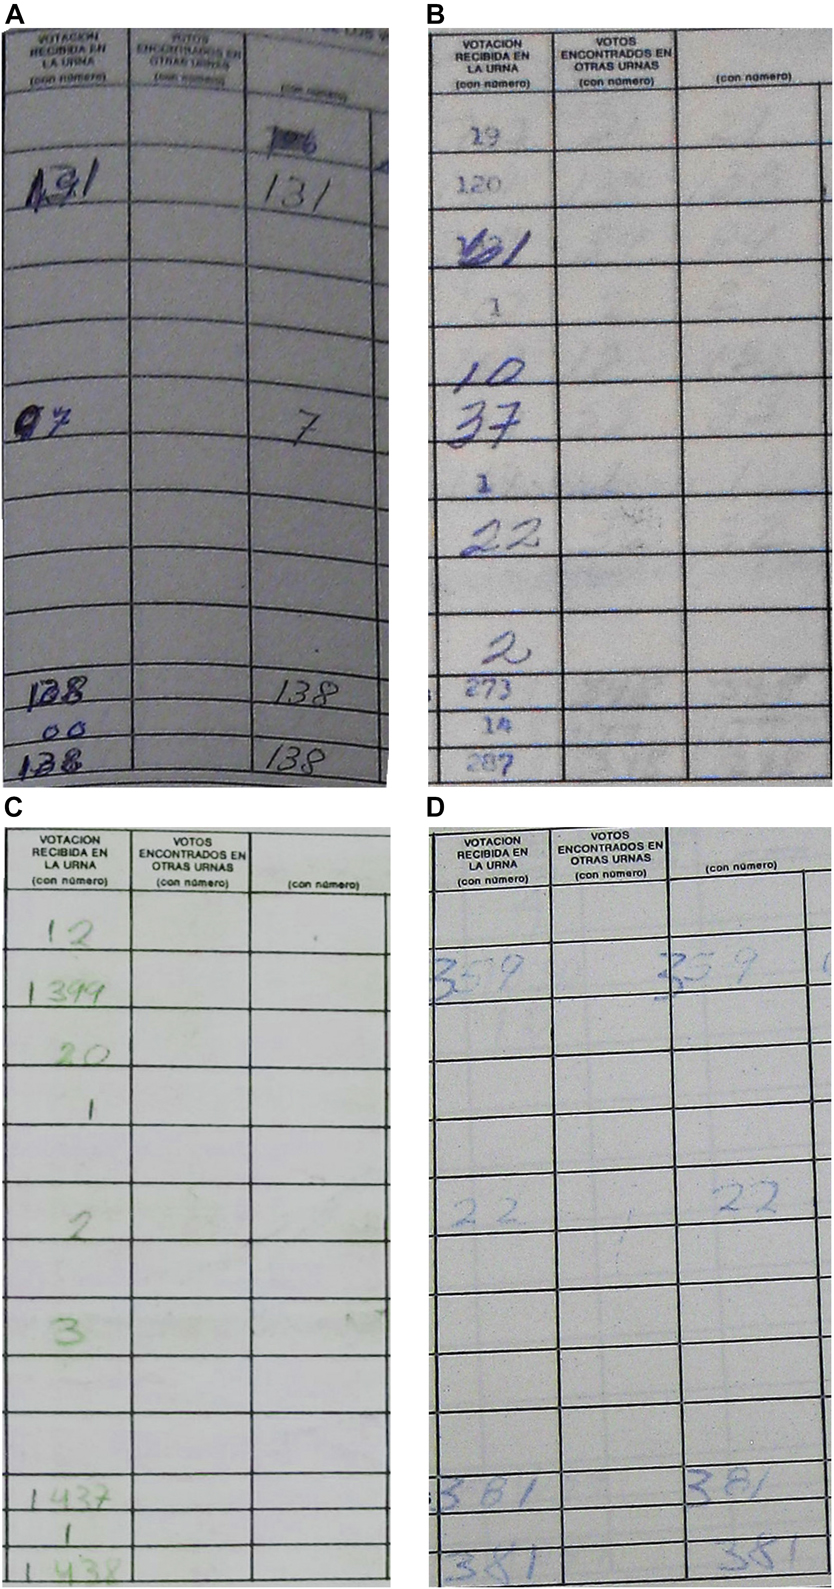
\includegraphics[width=2.70833in,height=\textheight]{image/fraud.png}
\caption{Examples of altered tally sheets (reproducing Figure 1 of Cantú
2018)}
\end{figure}

\clearpage

\hypertarget{task-0.-loading-required-packages-3pt}{%
\subsection{Task 0. Loading required packages
(3pt)}\label{task-0.-loading-required-packages-3pt}}

For Better organization, it is a good habit to load all required
packages up front at the start of your document. Please load the all
packages you use throughout the whole Problem Set here.

\begin{Shaded}
\begin{Highlighting}[]
\FunctionTok{library}\NormalTok{(tidyverse)}
\FunctionTok{library}\NormalTok{(ggplot2)}
\FunctionTok{library}\NormalTok{(dplyr)}
\end{Highlighting}
\end{Shaded}

\clearpage

\hypertarget{task-1.-clean-machine-classification-results-3pt}{%
\subsection{Task 1. Clean machine classification results
(3pt)}\label{task-1.-clean-machine-classification-results-3pt}}

Cantú applys machine learning models to 55,334 images of tally sheets to
detect signs of fraud (i.e., alteration). The machine learning model
returns results recorded in a table. The information in this table is
messy and requires data wrangling before we can use them.

\hypertarget{task-1.1.-load-classified-images-of-tally-sheets}{%
\subsubsection{Task 1.1. Load classified images of tally
sheets}\label{task-1.1.-load-classified-images-of-tally-sheets}}

The path of the classified images of tally sheets is
\texttt{data/classification.txt}. Your first task is loading these data
onto R using a \texttt{tidyverse} function. Name it \texttt{d\_tally}.

Note:

\begin{itemize}
\item
  Although the file extension of this dataset is \texttt{.txt}, you are
  recommended to use the \texttt{tidyverse} function we use for
  \texttt{.csv} files to read it.
\item
  Unlike the data files we have read in class, this table has \emph{no
  column names}. Look up the documentation and find a way to handle it.
\item
  There will be three columns in this dataset, name them
  \texttt{name\_image}, \texttt{label}, and \texttt{probability}.
\end{itemize}

Print your table to show your output.

\begin{Shaded}
\begin{Highlighting}[]
\CommentTok{\#Load the data }
\NormalTok{d\_tally}\OtherTok{\textless{}{-}}\FunctionTok{read.csv}\NormalTok{(}\StringTok{"data/classification.txt"}\NormalTok{, }\AttributeTok{header=}\ConstantTok{FALSE}\NormalTok{)}
\CommentTok{\#Rename of colomns }
\NormalTok{d\_tally}\OtherTok{\textless{}{-}}\NormalTok{d\_tally}\SpecialCharTok{|\textgreater{}}
       \FunctionTok{rename}\NormalTok{(}\StringTok{"name\_image"}\OtherTok{=}\NormalTok{ V1, }\StringTok{"label"}\OtherTok{=}\NormalTok{V2, }\StringTok{"probability"}\OtherTok{=}\NormalTok{V3)}
\FunctionTok{library}\NormalTok{(dplyr)}
\FunctionTok{tibble}\NormalTok{(d\_tally)}
\end{Highlighting}
\end{Shaded}

\begin{verbatim}
## # A tibble: 55,334 x 3
##    name_image                               label probability    
##    <chr>                                    <chr> <chr>          
##  1 Aguascalientes_I_2014-05-26 00.00.10.jpg [[0]] [[ 0.99919599]]
##  2 Aguascalientes_I_2014-05-26 00.00.17.jpg [[0]] [[ 0.95722806]]
##  3 Aguascalientes_I_2014-05-26 00.00.25.jpg [[0]] [[ 0.57690716]]
##  4 Aguascalientes_I_2014-05-26 00.00.31.jpg [[0]] [[ 0.96505082]]
##  5 Aguascalientes_I_2014-05-26 00.00.38.jpg [[0]] [[ 0.86975688]]
##  6 Aguascalientes_I_2014-05-26 00.00.45.jpg [[0]] [[ 0.78825063]]
##  7 Aguascalientes_I_2014-05-26 00.00.52.jpg [[0]] [[ 0.96493018]]
##  8 Aguascalientes_I_2014-05-26 00.00.59.jpg [[0]] [[ 0.68087846]]
##  9 Aguascalientes_I_2014-05-26 00.01.06.jpg [[0]] [[ 0.99999994]]
## 10 Aguascalientes_I_2014-05-26 00.01.15.jpg [[0]] [[ 0.64047635]]
## # i 55,324 more rows
\end{verbatim}

\clearpage

\hypertarget{note-1.-what-are-in-this-dataset}{%
\subsubsection{Note 1. What are in this
dataset?}\label{note-1.-what-are-in-this-dataset}}

Before you proceed, let me explain the meaning of the three variables.

\begin{itemize}
\item
  \texttt{name\_image} contains the names of of the tallies' image files
  (as you may infer from the \texttt{.jpg} file extensions. They contain
  information about the locations where each of the tally sheets are
  produced.
\item
  \texttt{label} is a machine-predicted label indicating whether a tally
  is fraudulent or not. \texttt{label\ =\ 1} means the machine learning
  model has detected signs of fraud in the tally sheet.
  \texttt{label\ =\ 0} means the machine detects no sign of fraud in the
  tally sheet. In short, \texttt{label\ =\ 1} means fraud;
  \texttt{label\ =\ 0} means no fraud.
\item
  \texttt{probability} indicates the machine's certainty about its
  predicted \texttt{label} (explained above). It ranges from 0 to 1,
  where higher values mean higher level of certainty.
\end{itemize}

Interpret \texttt{label} and \texttt{probability} carefully. Two
examples can hopefully give you clues about their correct
interpretation. In the first row, \texttt{label\ =\ 0} and
\texttt{probability\ =\ 0.9991}. That means the machine thinks this
tally sheet is NOT FRAUDULENT with a probability of 0.9991. Then, the
probability that this tally sheet is fraudulent is
\texttt{1\ -\ 0.9991\ =\ 0.0009}. Take another example, in the 11th row,
\texttt{label\ =\ 1} and \texttt{probability\ =\ 0.935}. This means the
machine thinks this tally sheet IS FRAUDULENT with a probability of
0.935. Then, the probability that it is NOT FRAUDULENT is
\texttt{1\ -\ 0.9354\ =\ 0.0646}.

\clearpage

\hypertarget{task-1.2.-clean-columns-label-and-probability}{%
\subsubsection{\texorpdfstring{Task 1.2. Clean columns \texttt{label}
and
\texttt{probability}}{Task 1.2. Clean columns label and probability}}\label{task-1.2.-clean-columns-label-and-probability}}

As you have seen in the printed outputs, columns \texttt{label} and
\texttt{probability} are read as \texttt{chr} variables when they are
actually numbers. A close look at the data may tell you why --- they are
``wrapped'' by some non-numeric characters. In this task, you will clean
these two variables and make them valid numeric variables. You are
required to use \texttt{tidyverse} operations to for this task. Show
appropriate summary statistics of \texttt{label} and
\texttt{probability} respectively after you have transformed them into
numeric variables.

\begin{Shaded}
\begin{Highlighting}[]
\CommentTok{\#Data cleaned}
\NormalTok{d\_tally}\OtherTok{\textless{}{-}}\NormalTok{ d\_tally}\SpecialCharTok{|\textgreater{}}
       \FunctionTok{mutate}\NormalTok{(}\AttributeTok{label =} \FunctionTok{as.numeric}\NormalTok{(}\FunctionTok{str\_remove\_all}\NormalTok{(label, }\StringTok{"}\SpecialCharTok{\textbackslash{}\textbackslash{}}\StringTok{[|}\SpecialCharTok{\textbackslash{}\textbackslash{}}\StringTok{]"}\NormalTok{)))}
\NormalTok{d\_tally}\OtherTok{\textless{}{-}}\NormalTok{d\_tally}\SpecialCharTok{|\textgreater{}} 
       \FunctionTok{mutate}\NormalTok{(}\AttributeTok{probability =} \FunctionTok{as.numeric}\NormalTok{(}\FunctionTok{str\_remove\_all}\NormalTok{(probability,}\StringTok{"}\SpecialCharTok{\textbackslash{}\textbackslash{}}\StringTok{[|}\SpecialCharTok{\textbackslash{}\textbackslash{}}\StringTok{]"}\NormalTok{)))}
\FunctionTok{tibble}\NormalTok{(d\_tally)}
\end{Highlighting}
\end{Shaded}

\begin{verbatim}
## # A tibble: 55,334 x 3
##    name_image                               label probability
##    <chr>                                    <dbl>       <dbl>
##  1 Aguascalientes_I_2014-05-26 00.00.10.jpg     0       0.999
##  2 Aguascalientes_I_2014-05-26 00.00.17.jpg     0       0.957
##  3 Aguascalientes_I_2014-05-26 00.00.25.jpg     0       0.577
##  4 Aguascalientes_I_2014-05-26 00.00.31.jpg     0       0.965
##  5 Aguascalientes_I_2014-05-26 00.00.38.jpg     0       0.870
##  6 Aguascalientes_I_2014-05-26 00.00.45.jpg     0       0.788
##  7 Aguascalientes_I_2014-05-26 00.00.52.jpg     0       0.965
##  8 Aguascalientes_I_2014-05-26 00.00.59.jpg     0       0.681
##  9 Aguascalientes_I_2014-05-26 00.01.06.jpg     0       1.00 
## 10 Aguascalientes_I_2014-05-26 00.01.15.jpg     0       0.640
## # i 55,324 more rows
\end{verbatim}

\begin{verbatim}
##    Min. 1st Qu.  Median    Mean 3rd Qu.    Max. 
##  0.0000  0.0000  0.0000  0.3623  1.0000  1.0000
\end{verbatim}

\begin{verbatim}
##    Min. 1st Qu.  Median    Mean 3rd Qu.    Max. 
##  0.5000  0.8185  0.9710  0.8926  0.9996  1.0000
\end{verbatim}

\clearpage

\hypertarget{task-1.3.-extract-state-and-district-information-from-name_image}{%
\subsubsection{\texorpdfstring{Task 1.3. Extract state and district
information from
\texttt{name\_image}}{Task 1.3. Extract state and district information from name\_image}}\label{task-1.3.-extract-state-and-district-information-from-name_image}}

As explained in the note, the column \texttt{name\_image}, which has the
names of tally sheets' images, contains information about locations
where the tally sheets are produced. Specifically, the first two
elements of these file names indicates the \textbf{states'} and
districts' identifiers respectively, for example,
\texttt{name\_image\ =\ "Aguascalientes\_I\_2014-05-26\ 00.00.10.jpg"}.
It means this tally sheet is produced in state
\textbf{\texttt{Aguascalientes}}, district \textbf{\texttt{I}}. In this
task, you are required to obtain this information. Specifically, create
two columns named \texttt{state} and \texttt{district} as state and
district identifiers respectively. You are required to use
\texttt{tidyverse} functions to perform the task.

\begin{Shaded}
\begin{Highlighting}[]
\NormalTok{ d\_tally}\OtherTok{\textless{}{-}}\NormalTok{ d\_tally}\SpecialCharTok{|\textgreater{}}
 \FunctionTok{mutate}\NormalTok{(}\AttributeTok{state =} \FunctionTok{str\_extract}\NormalTok{(name\_image, }\StringTok{"\^{}[A{-}Za{-}z]+"}\NormalTok{),}
         \AttributeTok{district =} \FunctionTok{str\_extract}\NormalTok{(name\_image, }\StringTok{"(?\textless{}=\_)[A{-}Za{-}z]+"}\NormalTok{))}
 
 \FunctionTok{tibble}\NormalTok{(d\_tally)}
\end{Highlighting}
\end{Shaded}

\begin{verbatim}
## # A tibble: 55,334 x 5
##    name_image                               label probability state     district
##    <chr>                                    <dbl>       <dbl> <chr>     <chr>   
##  1 Aguascalientes_I_2014-05-26 00.00.10.jpg     0       0.999 Aguascal~ I       
##  2 Aguascalientes_I_2014-05-26 00.00.17.jpg     0       0.957 Aguascal~ I       
##  3 Aguascalientes_I_2014-05-26 00.00.25.jpg     0       0.577 Aguascal~ I       
##  4 Aguascalientes_I_2014-05-26 00.00.31.jpg     0       0.965 Aguascal~ I       
##  5 Aguascalientes_I_2014-05-26 00.00.38.jpg     0       0.870 Aguascal~ I       
##  6 Aguascalientes_I_2014-05-26 00.00.45.jpg     0       0.788 Aguascal~ I       
##  7 Aguascalientes_I_2014-05-26 00.00.52.jpg     0       0.965 Aguascal~ I       
##  8 Aguascalientes_I_2014-05-26 00.00.59.jpg     0       0.681 Aguascal~ I       
##  9 Aguascalientes_I_2014-05-26 00.01.06.jpg     0       1.00  Aguascal~ I       
## 10 Aguascalientes_I_2014-05-26 00.01.15.jpg     0       0.640 Aguascal~ I       
## # i 55,324 more rows
\end{verbatim}

\clearpage

\hypertarget{task-1.4.-re-code-a-states-name}{%
\subsubsection{Task 1.4. Re-code a state's
name}\label{task-1.4.-re-code-a-states-name}}

One of the states (in the newly created column \texttt{state}) is coded
as ``\texttt{Estado\ de\ Mexico}.'' The researchers decide that it
should instead re-coded as ``\textbf{\texttt{Edomex}}.'' Please use a
\texttt{tidyverse} function to perform this task.

Hint: Look up functions \texttt{ifelse} and \texttt{case\_match}.

\begin{Shaded}
\begin{Highlighting}[]
\NormalTok{d\_tally}\OtherTok{\textless{}{-}}\NormalTok{ d\_tally}\SpecialCharTok{|\textgreater{}}
  \FunctionTok{mutate}\NormalTok{(}\AttributeTok{state =} \FunctionTok{ifelse}\NormalTok{(state }\SpecialCharTok{==} \StringTok{"Estado de Mexico"}\NormalTok{, }\StringTok{"Edomex"}\NormalTok{, state))}

\FunctionTok{tibble}\NormalTok{(d\_tally)}
\end{Highlighting}
\end{Shaded}

\begin{verbatim}
## # A tibble: 55,334 x 5
##    name_image                               label probability state     district
##    <chr>                                    <dbl>       <dbl> <chr>     <chr>   
##  1 Aguascalientes_I_2014-05-26 00.00.10.jpg     0       0.999 Aguascal~ I       
##  2 Aguascalientes_I_2014-05-26 00.00.17.jpg     0       0.957 Aguascal~ I       
##  3 Aguascalientes_I_2014-05-26 00.00.25.jpg     0       0.577 Aguascal~ I       
##  4 Aguascalientes_I_2014-05-26 00.00.31.jpg     0       0.965 Aguascal~ I       
##  5 Aguascalientes_I_2014-05-26 00.00.38.jpg     0       0.870 Aguascal~ I       
##  6 Aguascalientes_I_2014-05-26 00.00.45.jpg     0       0.788 Aguascal~ I       
##  7 Aguascalientes_I_2014-05-26 00.00.52.jpg     0       0.965 Aguascal~ I       
##  8 Aguascalientes_I_2014-05-26 00.00.59.jpg     0       0.681 Aguascal~ I       
##  9 Aguascalientes_I_2014-05-26 00.01.06.jpg     0       1.00  Aguascal~ I       
## 10 Aguascalientes_I_2014-05-26 00.01.15.jpg     0       0.640 Aguascal~ I       
## # i 55,324 more rows
\end{verbatim}

\clearpage

\hypertarget{task-1.5.-create-a-probability-of-fraud-indicator}{%
\subsubsection{\texorpdfstring{Task 1.5. Create a \emph{probability of
fraud}
indicator}{Task 1.5. Create a probability of fraud indicator}}\label{task-1.5.-create-a-probability-of-fraud-indicator}}

As explained in Note 1, we need to interpret label and probability with
caution, as the meaning of probability is conditional on the value of
label. To avoid confusion in the analysis, your next task is to create a
column named fraud\_proba which indicates the probability that a tally
sheet is is fraudulent. After you have created the column, drop the
label and probability columns.

Hint: Look up the ifelse function and the case\_when function (but you
just need either one of them).

\begin{Shaded}
\begin{Highlighting}[]
\CommentTok{\#Creation of the new column "fraud\_proba"}
\NormalTok{d\_tally }\OtherTok{\textless{}{-}}\NormalTok{ d\_tally }\SpecialCharTok{|\textgreater{}}
  \FunctionTok{mutate}\NormalTok{(}\AttributeTok{fraud\_proba =} \FunctionTok{ifelse}\NormalTok{(label }\SpecialCharTok{==} \DecValTok{1}\NormalTok{, probability, }\DecValTok{1} \SpecialCharTok{{-}}\NormalTok{ probability))}
\CommentTok{\#Dropping the label and probability columns}
\NormalTok{d\_tally }\OtherTok{\textless{}{-}} \FunctionTok{select}\NormalTok{(d\_tally, }\SpecialCharTok{{-}}\NormalTok{label, }\SpecialCharTok{{-}}\NormalTok{probability)}
\FunctionTok{tibble}\NormalTok{(d\_tally)}
\end{Highlighting}
\end{Shaded}

\begin{verbatim}
## # A tibble: 55,334 x 4
##    name_image                               state          district  fraud_proba
##    <chr>                                    <chr>          <chr>           <dbl>
##  1 Aguascalientes_I_2014-05-26 00.00.10.jpg Aguascalientes I        0.000804    
##  2 Aguascalientes_I_2014-05-26 00.00.17.jpg Aguascalientes I        0.0428      
##  3 Aguascalientes_I_2014-05-26 00.00.25.jpg Aguascalientes I        0.423       
##  4 Aguascalientes_I_2014-05-26 00.00.31.jpg Aguascalientes I        0.0349      
##  5 Aguascalientes_I_2014-05-26 00.00.38.jpg Aguascalientes I        0.130       
##  6 Aguascalientes_I_2014-05-26 00.00.45.jpg Aguascalientes I        0.212       
##  7 Aguascalientes_I_2014-05-26 00.00.52.jpg Aguascalientes I        0.0351      
##  8 Aguascalientes_I_2014-05-26 00.00.59.jpg Aguascalientes I        0.319       
##  9 Aguascalientes_I_2014-05-26 00.01.06.jpg Aguascalientes I        0.0000000600
## 10 Aguascalientes_I_2014-05-26 00.01.15.jpg Aguascalientes I        0.360       
## # i 55,324 more rows
\end{verbatim}

\clearpage

\hypertarget{task-1.6.-create-a-binary-fraud-indicator}{%
\subsubsection{\texorpdfstring{Task 1.6. Create a binary \emph{fraud}
indicator}{Task 1.6. Create a binary fraud indicator}}\label{task-1.6.-create-a-binary-fraud-indicator}}

In this task, you will create a binary indicator called
\texttt{fraud\_bin} in indicating whether a tally sheet is fraudulent.
Following the researcher's rule, we consider a tally sheet fraudulent
only when the machine thinks it is at least 2/3 likely to be fraudulent.
That is, \texttt{fraud\_bin} is set to TRUE when \texttt{fraud\_proba}
is greater to \texttt{2/3} and is FALSE otherwise.

\begin{Shaded}
\begin{Highlighting}[]
\NormalTok{d\_tally}\OtherTok{\textless{}{-}}\NormalTok{ d\_tally }\SpecialCharTok{|\textgreater{}}
  \FunctionTok{mutate}\NormalTok{(}\AttributeTok{fraud\_bin =} \FunctionTok{ifelse}\NormalTok{(fraud\_proba }\SpecialCharTok{\textgreater{}=} \DecValTok{2}\SpecialCharTok{/}\DecValTok{3}\NormalTok{, }\ConstantTok{TRUE}\NormalTok{, }\ConstantTok{FALSE}\NormalTok{))}
\FunctionTok{tibble}\NormalTok{(d\_tally)}
\end{Highlighting}
\end{Shaded}

\begin{verbatim}
## # A tibble: 55,334 x 5
##    name_image                               state district fraud_proba fraud_bin
##    <chr>                                    <chr> <chr>          <dbl> <lgl>    
##  1 Aguascalientes_I_2014-05-26 00.00.10.jpg Agua~ I            8.04e-4 FALSE    
##  2 Aguascalientes_I_2014-05-26 00.00.17.jpg Agua~ I            4.28e-2 FALSE    
##  3 Aguascalientes_I_2014-05-26 00.00.25.jpg Agua~ I            4.23e-1 FALSE    
##  4 Aguascalientes_I_2014-05-26 00.00.31.jpg Agua~ I            3.49e-2 FALSE    
##  5 Aguascalientes_I_2014-05-26 00.00.38.jpg Agua~ I            1.30e-1 FALSE    
##  6 Aguascalientes_I_2014-05-26 00.00.45.jpg Agua~ I            2.12e-1 FALSE    
##  7 Aguascalientes_I_2014-05-26 00.00.52.jpg Agua~ I            3.51e-2 FALSE    
##  8 Aguascalientes_I_2014-05-26 00.00.59.jpg Agua~ I            3.19e-1 FALSE    
##  9 Aguascalientes_I_2014-05-26 00.01.06.jpg Agua~ I            6.00e-8 FALSE    
## 10 Aguascalientes_I_2014-05-26 00.01.15.jpg Agua~ I            3.60e-1 FALSE    
## # i 55,324 more rows
\end{verbatim}

\clearpage

\hypertarget{task-2.-visualize-machine-classification-results-3pt}{%
\subsection{Task 2. Visualize machine classification results
(3pt)}\label{task-2.-visualize-machine-classification-results-3pt}}

In this section, you will visualize the \texttt{tally} dataset that you
have cleaned in Task 1. Unless otherwise specified, you are required to
use the \texttt{ggplot} packages to perform all the tasks.

\hypertarget{task-2.1.-visualize-distribution-of-fraud_proba}{%
\subsubsection{\texorpdfstring{Task 2.1. Visualize distribution of
\texttt{fraud\_proba}}{Task 2.1. Visualize distribution of fraud\_proba}}\label{task-2.1.-visualize-distribution-of-fraud_proba}}

How is the predicted probability of fraud (\texttt{fraud\_proba})
distributed? Use two methods to visualize the distribution. Remember to
add informative labels to the figure. Describe the plot with a few
sentences.

\begin{Shaded}
\begin{Highlighting}[]
\CommentTok{\#Method1:Histogram }
\FunctionTok{ggplot}\NormalTok{(d\_tally, }\FunctionTok{aes}\NormalTok{(}\AttributeTok{x =}\NormalTok{ fraud\_proba)) }\SpecialCharTok{+}
  \FunctionTok{geom\_histogram}\NormalTok{(}\AttributeTok{fill =} \StringTok{"steelblue"}\NormalTok{, }\AttributeTok{color =} \StringTok{"white"}\NormalTok{) }\SpecialCharTok{+}
  \FunctionTok{labs}\NormalTok{(}\AttributeTok{title =} \StringTok{"Distribution of Predicted Probability of Fraud"}\NormalTok{,}
       \AttributeTok{x =} \StringTok{"Predicted Probability of Fraud"}\NormalTok{,}
       \AttributeTok{y =} \StringTok{"Count"}\NormalTok{)}
\end{Highlighting}
\end{Shaded}

\begin{center}\includegraphics[width=0.5\linewidth]{POLI3148_PS_answer_[3035945883]_files/figure-latex/unnamed-chunk-9-1} \end{center}

Description: This histogram shows that those tally sheets with 0
probability of fraudulent has the highest frequency, reaching around
17500 counts.The second highest count is 7500, which stands for the
count of tally sheets with the probability of fraudulent equals to 1.
The count of the tally sheets with probability of fraudulent between 0
and 1 is relatively lower than fraud\_proba = 0 or 1. The fluctuations
of count remain between 3750 and 625, and the distribution is uniform.

\includegraphics{POLI3148_PS_answer_{[}3035945883{]}_files/figure-latex/unnamed-chunk-10-1.pdf}

Description: The density plot has a shape similar with the histogram.
The density of tally sheets with probability of fraudulent close to 0 is
the highest at around 3.6, and those tally sheets with the probability
of fraudulent close to 1, the density is 1.8. Also, the count of tally
sheets with probability of fraud between 0 and1 is relatively lower and
the distribution is uniform without large fluctuations.

\clearpage

\hypertarget{task-2.2.-visualize-distribution-of-fraud_bin}{%
\subsubsection{\texorpdfstring{Task 2.2. Visualize distribution of
\texttt{fraud\_bin}}{Task 2.2. Visualize distribution of fraud\_bin}}\label{task-2.2.-visualize-distribution-of-fraud_bin}}

How many tally sheets are fraudulent and how many are not? We may answer
this question by visualizing the binary indicator of tally-level states
of fraud. Use at least two methods to visualize the distribution of
\texttt{fraud\_bin}. Remember to add informative labels to the figure.
Describe your plots with a few sentences.

\begin{Shaded}
\begin{Highlighting}[]
\CommentTok{\# Method1:Bar chart }
\FunctionTok{ggplot}\NormalTok{(d\_tally, }\FunctionTok{aes}\NormalTok{(}\AttributeTok{x =}\NormalTok{ fraud\_bin)) }\SpecialCharTok{+}
  \FunctionTok{geom\_bar}\NormalTok{(}\AttributeTok{fill =} \StringTok{"steelblue"}\NormalTok{, }\AttributeTok{color =} \StringTok{"white"}\NormalTok{) }\SpecialCharTok{+}
  \FunctionTok{labs}\NormalTok{(}\AttributeTok{title =} \StringTok{"Distribution of Tally{-}Level States of Fraud"}\NormalTok{,}
       \AttributeTok{x =} \StringTok{"Fraudulent"}\NormalTok{,}
       \AttributeTok{y =} \StringTok{"Count"}\NormalTok{) }\SpecialCharTok{+}
  \FunctionTok{scale\_x\_discrete}\NormalTok{(}\AttributeTok{labels =} \FunctionTok{c}\NormalTok{(}\StringTok{"Not Fraud"}\NormalTok{, }\StringTok{"Fraud"}\NormalTok{))}
\end{Highlighting}
\end{Shaded}

\begin{center}\includegraphics[width=0.5\linewidth]{POLI3148_PS_answer_[3035945883]_files/figure-latex/unnamed-chunk-11-1} \end{center}

Description: The bar chart shows the two categories as ``fraud'' and
``not fraud'',there is around 17000 tally sheets are identified as
fraud. Also, the count of tally sheetes which are identified as not
fraud is more than twice of those identified as fraud.

\includegraphics{POLI3148_PS_answer_{[}3035945883{]}_files/figure-latex/unnamed-chunk-12-1.pdf}

Description: The pie chart vividly shows that there is around 1/3 of the
tally sheets are identified as fraud, and the left tally sheets are not.

The figure below serve as a reference. Feel free to try alternative
approach(es) to make your visualization nicer and more informative.

\clearpage

\hypertarget{task-2.3.-summarize-prevalence-of-fraud-by-state}{%
\subsubsection{Task 2.3. Summarize prevalence of fraud by
state}\label{task-2.3.-summarize-prevalence-of-fraud-by-state}}

Next, we will examine the between-state variation with regards to the
prevalence of election fraud. In this task, you will create a new object
that contains two state-level indicators regarding the prevalence of
election fraud: The count of fraudulent tallies and the proportion of
fraudulent tallies.

\begin{Shaded}
\begin{Highlighting}[]
\NormalTok{d\_state}\OtherTok{\textless{}{-}}\NormalTok{ d\_tally }\SpecialCharTok{|\textgreater{}}
  \FunctionTok{group\_by}\NormalTok{(state) }\SpecialCharTok{|\textgreater{}}
  \FunctionTok{summarize}\NormalTok{(}\AttributeTok{fraud\_count =} \FunctionTok{sum}\NormalTok{(fraud\_bin),}
            \AttributeTok{fraud\_prop =} \FunctionTok{mean}\NormalTok{(fraud\_bin))}
\FunctionTok{tibble}\NormalTok{(d\_state)}
\end{Highlighting}
\end{Shaded}

\begin{verbatim}
## # A tibble: 31 x 3
##    state          fraud_count fraud_prop
##    <chr>                <int>      <dbl>
##  1 Aguascalientes          71     0.176 
##  2 Baja                   390     0.221 
##  3 Campeche               146     0.386 
##  4 Chiapas                629     0.456 
##  5 Chihuahua              398     0.214 
##  6 Coahuila               444     0.378 
##  7 Colima                  51     0.168 
##  8 Distrito               236     0.0310
##  9 Durango                376     0.278 
## 10 Estado                 256     0.0603
## # i 21 more rows
\end{verbatim}

\clearpage

\hypertarget{task-2.4.-visualize-frequencies-of-fraud-by-state}{%
\subsubsection{Task 2.4. Visualize frequencies of fraud by
state}\label{task-2.4.-visualize-frequencies-of-fraud-by-state}}

Using the new data frame created in Task 2.3, please visualize the
\emph{frequencies} of fraudulent tallies of every state. Describe the
key takeaway from the visualization with a few sentences.

Feel free to try alternative approach(es) to make your visualization
nicer and more informative.

\includegraphics{POLI3148_PS_answer_{[}3035945883{]}_files/figure-latex/unnamed-chunk-14-1.pdf}

Description: All of the states have tally sheets identitifes as fraud.
The tally cheetes from Veracruz has the most counts of fraudulent, and
the frequency reaches 2250. In contrast, Quintana, Hidalgo and Colima
has much less fraud tally sheets.

\clearpage

\hypertarget{task-2.5.-visualize-proportions-of-fraud-by-state}{%
\subsubsection{Task 2.5. Visualize proportions of fraud by
state}\label{task-2.5.-visualize-proportions-of-fraud-by-state}}

Using the new data frame created in Task 2.3, please visualize the
\emph{proportion of} of fraudulent tallies of every state. Describe the
key takeaway from the visualization with a few sentences.

Feel free to try alternative approach(es) to make your visualization
nicer and more informative.

\includegraphics{POLI3148_PS_answer_{[}3035945883{]}_files/figure-latex/unnamed-chunk-15-1.pdf}

Description: The proportion of fraudulent tallies in ten states reaches
0.5, as the right red line splitted. The state with lowest proportion of
fraudulent tallies is Distrito, and the left red line shows that there
are three states with proportion of draudulent tallies under 0.1.

\clearpage

\hypertarget{task-2.6.-visualize-both-proportions-frequencies-of-fraud-by-state}{%
\subsubsection{Task 2.6. Visualize both proportions \& frequencies of
fraud by
state}\label{task-2.6.-visualize-both-proportions-frequencies-of-fraud-by-state}}

Create data visualization to show BOTH the \emph{proportions} and
\emph{frequencies} of fraudulent tally sheets by state in one figure.
Include annotations to highlight states with the highest level of fraud.
Add informative labels to the figure. Describe the takeaways from the
figure with a few sentences.

\begin{Shaded}
\begin{Highlighting}[]
\CommentTok{\#d\_tally \textless{}{-} d\_tally |\textgreater{}}
  \CommentTok{\#arrange(desc(fraud\_prop)) |\textgreater{}}
  \CommentTok{\#mutate(state = factor(state, levels = state))}

\CommentTok{\# Create the stacked bar chart}
\CommentTok{\#ggplot(d\_tally, aes(x = state, y = fraud\_count, fill = fraud\_count)) +}
  \CommentTok{\#geom\_bar(stat = "identity", position = "stack") +}
  \CommentTok{\#labs(x = "State", y = "Number of Fraudulent Tally Sheets", fill = "Fraudulent") +}
  \CommentTok{\#theme\_minimal() +}
  \CommentTok{\#theme(axis.text.x = element\_text(angle = 45, hjust = 1)) +}
  \CommentTok{\#ggtitle("Fraudulent Tally Sheets by State") +}
  \CommentTok{\#geom\_text(aes(label = fraud\_count), vjust = {-}0.5, color = "black", size = 3.5) +}
  \CommentTok{\#geom\_text(aes(label = sprintf("\%.2f", fraud\_prop)), vjust = 1.5, color = "black", size = 3.5) +}
  \CommentTok{\#annotate("text", x = which.max(d\_tally$fraud\_count), y = max(d\_tally$fraud\_count) + 10, }
           \CommentTok{\#label = "Highest fraud count", vjust = 0, hjust = 0, color = "black") +}
  \CommentTok{\#annotate("text", x = which.max(d\_tally$fraud\_pro), y = max(d\_tally$fraud\_count) + 10, }
           \CommentTok{\#label = "Highest fraud proportion", vjust = 0, hjust = 1, color = "black")}
\end{Highlighting}
\end{Shaded}

Description:

\clearpage

\hypertarget{task-3.-clean-vote-return-data-3pt}{%
\subsection{Task 3. Clean vote return data
(3pt)}\label{task-3.-clean-vote-return-data-3pt}}

Your next task is to clean a different dataset from the researchers'
replication dossier. Its path is
\texttt{data/Mexican\_Election\_Fraud/dataverse/VoteReturns.csv}. This
dataset contains information about vote returns recorded in every tally
sheet. This dataset is essential for the replication of Figure 4 in the
research article.

\hypertarget{task-3.1.-load-vote-return-data}{%
\subsubsection{Task 3.1. Load vote return
data}\label{task-3.1.-load-vote-return-data}}

Load the dataset onto your R environment. Name this dataset
\texttt{d\_return}. Show summary statistics of this dataset and describe
the takeaways using a few sentences.

\begin{Shaded}
\begin{Highlighting}[]
\NormalTok{d\_return}\OtherTok{\textless{}{-}} \FunctionTok{read.csv}\NormalTok{(}\StringTok{"data/VoteReturns.csv"}\NormalTok{)}
\FunctionTok{summary}\NormalTok{(d\_return)}
\end{Highlighting}
\end{Shaded}

\begin{verbatim}
##      foto             seccion            casilla              dtto          
##  Length:53499       Length:53499       Length:53499       Length:53499      
##  Class :character   Class :character   Class :character   Class :character  
##  Mode  :character   Mode  :character   Mode  :character   Mode  :character  
##                                                                             
##                                                                             
##                                                                             
##                                                                             
##       dto           municipio             edo              entidad         
##  Min.   :  1.000   Length:53499       Length:53499       Length:53499      
##  1st Qu.:  3.000   Class :character   Class :character   Class :character  
##  Median :  6.000   Mode  :character   Mode  :character   Mode  :character  
##  Mean   :  8.704                                                           
##  3rd Qu.: 10.000                                                           
##  Max.   :341.000                                                           
##  NA's   :4                                                                 
##     pagina                p1                 p2                p3        
##  Length:53499       Min.   :     0.0   Min.   :    0.0   Min.   :   0.0  
##  Class :character   1st Qu.:   250.0   1st Qu.:   67.0   1st Qu.:  98.0  
##  Mode  :character   Median :   530.0   Median :  245.0   Median : 233.0  
##                     Mean   :   671.9   Mean   :  343.3   Mean   : 319.3  
##                     3rd Qu.:   941.5   3rd Qu.:  482.0   3rd Qu.: 442.0  
##                     Max.   :364105.0   Max.   :48225.0   Max.   :9127.0  
##                                                          NA's   :1       
##        p4                p5               pan               pri        
##  Min.   :    0.0   Min.   :   0.00   Min.   :   0.00   Min.   :   0.0  
##  1st Qu.:   73.0   1st Qu.:   0.00   1st Qu.:   2.00   1st Qu.:  52.0  
##  Median :  222.0   Median :  13.00   Median :  18.00   Median : 107.0  
##  Mean   :  369.7   Mean   :  29.36   Mean   :  56.88   Mean   : 162.7  
##  3rd Qu.:  464.0   3rd Qu.:  36.00   3rd Qu.:  72.00   3rd Qu.: 195.0  
##  Max.   :21265.0   Max.   :6650.00   Max.   :4436.00   Max.   :6080.0  
##                                                                        
##       pps               psm                pms              pfcrn        
##  Min.   :   0.00   Min.   :   0.000   Min.   :   0.00   Min.   :   0.00  
##  1st Qu.:   0.00   1st Qu.:   0.000   1st Qu.:   0.00   1st Qu.:   0.00  
##  Median :   9.00   Median :   1.000   Median :   2.00   Median :  11.00  
##  Mean   :  35.04   Mean   :   3.637   Mean   :  12.19   Mean   :  34.17  
##  3rd Qu.:  47.00   3rd Qu.:   3.000   3rd Qu.:  13.00   3rd Qu.:  45.00  
##  Max.   :1056.00   Max.   :1802.000   Max.   :5511.00   Max.   :1011.00  
##                                                                          
##       prt               parm            noregis           nombrenore       
##  Min.   :  0.000   Min.   :   0.00   Min.   :   0.0000   Length:53499      
##  1st Qu.:  0.000   1st Qu.:   0.00   1st Qu.:   0.0000   Class :character  
##  Median :  0.000   Median :   5.00   Median :   0.0000   Mode  :character  
##  Mean   :  1.912   Mean   :  20.44   Mean   :   0.8175                     
##  3rd Qu.:  1.000   3rd Qu.:  23.00   3rd Qu.:   0.0000                     
##  Max.   :592.000   Max.   :1170.00   Max.   :1604.0000                     
##                                      NA's   :1                             
##      otros            otroscan              pan2               pri2         
##  Min.   :   0.000   Length:53499       Min.   :   0.000   Min.   :   0.000  
##  1st Qu.:   0.000   Class :character   1st Qu.:   0.000   1st Qu.:   0.000  
##  Median :   0.000   Mode  :character   Median :   0.000   Median :   0.000  
##  Mean   :   3.171                      Mean   :   1.475   Mean   :   3.941  
##  3rd Qu.:   0.000                      3rd Qu.:   0.000   3rd Qu.:   0.000  
##  Max.   :1734.000                      Max.   :1239.000   Max.   :2651.000  
##  NA's   :4                                                                  
##       pps2               psm2              pms2              pfcrn2         
##  Min.   :  0.0000   Min.   :  0.000   Min.   :  0.0000   Min.   :   0.0000  
##  1st Qu.:  0.0000   1st Qu.:  0.000   1st Qu.:  0.0000   1st Qu.:   0.0000  
##  Median :  0.0000   Median :  0.000   Median :  0.0000   Median :   0.0000  
##  Mean   :  0.7557   Mean   :  0.116   Mean   :  0.3039   Mean   :   0.7968  
##  3rd Qu.:  0.0000   3rd Qu.:  0.000   3rd Qu.:  0.0000   3rd Qu.:   0.0000  
##  Max.   :680.0000   Max.   :429.000   Max.   :427.0000   Max.   :1319.0000  
##                                                                             
##       prt2             parm2             noregis2             otro2          
##  Min.   :  0.000   Min.   :  0.0000   Min.   :  0.00000   Min.   : 0.000000  
##  1st Qu.:  0.000   1st Qu.:  0.0000   1st Qu.:  0.00000   1st Qu.: 0.000000  
##  Median :  0.000   Median :  0.0000   Median :  0.00000   Median : 0.000000  
##  Mean   :  0.073   Mean   :  0.5122   Mean   :  0.01837   Mean   : 0.002935  
##  3rd Qu.:  0.000   3rd Qu.:  0.0000   3rd Qu.:  0.00000   3rd Qu.: 0.000000  
##  Max.   :429.000   Max.   :429.0000   Max.   :259.00000   Max.   :26.000000  
##                                                                              
##       pan3              pri3             pps3             psm3        
##  Min.   :   0.00   Min.   :   0.0   Min.   :  0.00   Min.   :  0.000  
##  1st Qu.:   0.00   1st Qu.:   0.0   1st Qu.:  0.00   1st Qu.:  0.000  
##  Median :   0.00   Median :  32.0   Median :  0.00   Median :  0.000  
##  Mean   :  39.36   Mean   :  93.5   Mean   : 22.08   Mean   :  2.094  
##  3rd Qu.:  45.00   3rd Qu.: 127.0   3rd Qu.: 21.00   3rd Qu.:  1.000  
##  Max.   :2194.00   Max.   :6080.0   Max.   :921.00   Max.   :856.000  
##                    NA's   :1                         NA's   :2        
##       pms3              pfcrn3            prt3             parm3        
##  Min.   :   0.000   Min.   :  0.00   Min.   :  0.000   Min.   :   0.00  
##  1st Qu.:   0.000   1st Qu.:  0.00   1st Qu.:  0.000   1st Qu.:   0.00  
##  Median :   0.000   Median :  0.00   Median :  0.000   Median :   0.00  
##  Mean   :   7.803   Mean   : 21.63   Mean   :  1.077   Mean   :  12.68  
##  3rd Qu.:   5.000   3rd Qu.: 23.00   3rd Qu.:  1.000   3rd Qu.:  11.00  
##  Max.   :8932.000   Max.   :992.00   Max.   :413.000   Max.   :1170.00  
##  NA's   :1          NA's   :1                                           
##     noregis3            otro3                suma            nulos        
##  Min.   :  0.0000   Min.   :   0.0000   Min.   :   0.0   Min.   :   0.00  
##  1st Qu.:  0.0000   1st Qu.:   0.0000   1st Qu.:  82.0   1st Qu.:   0.00  
##  Median :  0.0000   Median :   0.0000   Median : 217.0   Median :   3.00  
##  Mean   :  0.3498   Mean   :   0.3016   Mean   : 296.4   Mean   :  21.93  
##  3rd Qu.:  0.0000   3rd Qu.:   0.0000   3rd Qu.: 420.0   3rd Qu.:  11.00  
##  Max.   :747.0000   Max.   :1353.0000   Max.   :9962.0   Max.   :8770.00  
##                     NA's   :1           NA's   :1        NA's   :1        
##      total             suma1              nulos1             total1        
##  Min.   :    0.0   Min.   :   0.000   Min.   :   0.000   Min.   :   0.000  
##  1st Qu.:   90.0   1st Qu.:   0.000   1st Qu.:   0.000   1st Qu.:   0.000  
##  Median :  229.0   Median :   0.000   Median :   0.000   Median :   0.000  
##  Mean   :  315.7   Mean   :   4.865   Mean   :   0.635   Mean   :   7.175  
##  3rd Qu.:  440.0   3rd Qu.:   0.000   3rd Qu.:   0.000   3rd Qu.:   0.000  
##  Max.   :16811.0   Max.   :3333.000   Max.   :1600.000   Max.   :2787.000  
##  NA's   :1         NA's   :2          NA's   :2          NA's   :2         
##      suma2            nulos2            total2         inciden         
##  Min.   :   0.0   Min.   :   0.00   Min.   :   0.0   Length:53499      
##  1st Qu.:   0.0   1st Qu.:   0.00   1st Qu.:   0.0   Class :character  
##  Median :   0.0   Median :   0.00   Median :   0.0   Mode  :character  
##  Mean   : 176.9   Mean   :  11.38   Mean   : 192.6                     
##  3rd Qu.: 280.0   3rd Qu.:   5.00   3rd Qu.: 299.0                     
##  Max.   :7633.0   Max.   :7734.00   Max.   :9855.0                     
##  NA's   :2        NA's   :2         NA's   :2                          
##  representante_pan  representante_pri  representante_pps  representante_pms 
##  Length:53499       Length:53499       Length:53499       Length:53499      
##  Class :character   Class :character   Class :character   Class :character  
##  Mode  :character   Mode  :character   Mode  :character   Mode  :character  
##                                                                             
##                                                                             
##                                                                             
##                                                                             
##  representante_psm  representante_pfcrn representante_prt  representante_parm
##  Length:53499       Length:53499        Length:53499       Length:53499      
##  Class :character   Class :character    Class :character   Class :character  
##  Mode  :character   Mode  :character    Mode  :character   Mode  :character  
##                                                                              
##                                                                              
##                                                                              
##                                                                              
##  protesta_pan       protesta_pri       protesta_pps       protesta_pms      
##  Length:53499       Length:53499       Length:53499       Length:53499      
##  Class :character   Class :character   Class :character   Class :character  
##  Mode  :character   Mode  :character   Mode  :character   Mode  :character  
##                                                                             
##                                                                             
##                                                                             
##                                                                             
##  protesta_psm       protesta_pfcrn     protesta_prt       protesta_parm     
##  Length:53499       Length:53499       Length:53499       Length:53499      
##  Class :character   Class :character   Class :character   Class :character  
##  Mode  :character   Mode  :character   Mode  :character   Mode  :character  
##                                                                             
##                                                                             
##                                                                             
##                                                                             
##  protesta_otro       presidente         secretario           primer         
##  Length:53499       Length:53499       Length:53499       Length:53499      
##  Class :character   Class :character   Class :character   Class :character  
##  Mode  :character   Mode  :character   Mode  :character   Mode  :character  
##                                                                             
##                                                                             
##                                                                             
##                                                                             
##    segundo            observa              var79           salinas      
##  Length:53499       Length:53499       Min.   :   1.0   Min.   :   0.0  
##  Class :character   Class :character   1st Qu.:   1.0   1st Qu.:  63.0  
##  Mode  :character   Mode  :character   Median :   1.0   Median : 115.0  
##                                        Mean   : 131.2   Mean   : 174.4  
##                                        3rd Qu.:   2.0   3rd Qu.: 206.0  
##                                        Max.   :9999.0   Max.   :6080.0  
##                                        NA's   :53422                    
##    clouthier           ibarra           castillo        ppsccs       
##  Min.   :   0.00   Min.   :  0.000   Min.   :   0   Min.   :   0.00  
##  1st Qu.:   3.00   1st Qu.:  0.000   1st Qu.:   0   1st Qu.:   1.00  
##  Median :  23.00   Median :  0.000   Median :   1   Median :  12.00  
##  Mean   :  61.37   Mean   :  2.185   Mean   :   4   Mean   :  37.67  
##  3rd Qu.:  78.00   3rd Qu.:  2.000   3rd Qu.:   3   3rd Qu.:  51.00  
##  Max.   :4436.00   Max.   :592.000   Max.   :1802   Max.   :1056.00  
##                                                                      
##     pfcrnccs          parmccs            nrccs             noregccs        
##  Min.   :   0.00   Min.   :   0.00   Min.   :0.000000   Min.   :   0.0000  
##  1st Qu.:   1.00   1st Qu.:   0.00   1st Qu.:0.000000   1st Qu.:   0.0000  
##  Median :  14.00   Median :   6.00   Median :0.000000   Median :   0.0000  
##  Mean   :  36.85   Mean   :  21.98   Mean   :0.006654   Mean   :   0.1439  
##  3rd Qu.:  48.00   3rd Qu.:  25.00   3rd Qu.:0.000000   3rd Qu.:   0.0000  
##  Max.   :1319.00   Max.   :1170.00   Max.   :1.000000   Max.   :1125.0000  
##                                                                            
##       occs           otrosccs           cardenas      
##  Min.   :0.0000   Min.   :   0.000   Min.   :   0.00  
##  1st Qu.:1.0000   1st Qu.:   0.000   1st Qu.:  10.00  
##  Median :1.0000   Median :   0.000   Median :  53.00  
##  Mean   :0.9942   Mean   :   3.106   Mean   :  99.75  
##  3rd Qu.:1.0000   3rd Qu.:   0.000   3rd Qu.: 141.00  
##  Max.   :1.0000   Max.   :1734.000   Max.   :2280.00  
## 
\end{verbatim}

\begin{Shaded}
\begin{Highlighting}[]
\FunctionTok{tibble}\NormalTok{(d\_return)}
\end{Highlighting}
\end{Shaded}

\begin{verbatim}
## # A tibble: 53,499 x 91
##    foto   seccion casilla dtto    dto municipio edo   entidad pagina    p1    p2
##    <chr>  <chr>   <chr>   <chr> <int> <chr>     <chr> <chr>   <chr>  <int> <int>
##  1 2014-~ 83      83      "I"       1 "AGUASCA~ Agua~ AGS     127      108   333
##  2 2014-~ 1       84      ""        1 "AGUASCA~ Agua~ AGUASC~ 128      919   453
##  3 2014-~ 85      85      "1"       1 "AGUASCA~ Agua~ AGUASC~ 129      795   264
##  4 2014-~ 45      45-A    "1"       1 "AGUASCA~ Agua~ AGUA    130      767   450
##  5 2014-~ 86      86      "1"       1 "AGUASCA~ Agua~ AGUAS   131     1243   578
##  6 2014-~ 87      87      "1"       1 ""        Agua~ 1       132      718   333
##  7 2014-~ 1       87-A    "7"       1 "AGUASCA~ Agua~ AGUAS   133      710   299
##  8 2014-~ 88      88      "1"       1 "AGUAS"   Agua~ AGUAS   134        0     0
##  9 2014-~ 89      89      "1"       1 "AGUASCA~ Agua~ AGUAS   135      764     8
## 10 2014-~ 89      89-A    "7"       1 "AGUSCAL~ Agua~ 1       136      759   256
## # i 53,489 more rows
## # i 80 more variables: p3 <int>, p4 <int>, p5 <int>, pan <int>, pri <int>,
## #   pps <int>, psm <int>, pms <int>, pfcrn <int>, prt <int>, parm <int>,
## #   noregis <int>, nombrenore <chr>, otros <int>, otroscan <chr>, pan2 <int>,
## #   pri2 <int>, pps2 <int>, psm2 <int>, pms2 <int>, pfcrn2 <int>, prt2 <int>,
## #   parm2 <int>, noregis2 <int>, otro2 <int>, pan3 <int>, pri3 <int>,
## #   pps3 <int>, psm3 <int>, pms3 <int>, pfcrn3 <int>, prt3 <int>, ...
\end{verbatim}

\clearpage

\hypertarget{note-2.-what-are-in-this-dataset}{%
\subsubsection{Note 2. What are in this
dataset?}\label{note-2.-what-are-in-this-dataset}}

This table contains a lot of different variables. The researcher offers
no comprehensive documentation to tell us what every column means. For
the sake of this problem set, you only need to know the meanings of the
following columns:

\begin{itemize}
\item
  \texttt{foto} is an identifier of the images of tally sheets in this
  dataset. We will need it to merge this dataset with the
  \texttt{d\_tally} data.
\item
  \texttt{edo} contains the names of states.
\item
  \texttt{dto} contains the names of districts (in Arabic numbers).
\item
  \texttt{salinas}, \texttt{clouthier}, and \texttt{ibarra} contain the
  counts of votes (as recorded in the tally sheets) for presidential
  candidates Salinas (PRI), Cardenas (FDN), and Clouthier (PAN). In
  addition, the summation of all three makes the total number of
  \textbf{presidential votes}.
\item
  \texttt{total} contains the total number of \textbf{legislative
  votes}.
\end{itemize}

\clearpage

\hypertarget{task-3.2.-recode-names-of-states}{%
\subsubsection{Task 3.2. Recode names of
states}\label{task-3.2.-recode-names-of-states}}

A state whose name is \texttt{Chihuahua} is mislabelled as
\texttt{Chihuhua}. A state whose name is currently \texttt{Edomex} needs
to be recoded to \texttt{Estado\ de\ Mexico}. Please re-code the names
of these two states accordingly.

\begin{Shaded}
\begin{Highlighting}[]
\FunctionTok{library}\NormalTok{(tidyverse)}
\NormalTok{d\_return }\OtherTok{\textless{}{-}}\NormalTok{ d\_return }\SpecialCharTok{|\textgreater{}}
  \FunctionTok{mutate}\NormalTok{(}\AttributeTok{edo =} \FunctionTok{case\_when}\NormalTok{(}
\NormalTok{    edo }\SpecialCharTok{==} \StringTok{"Chihuhua"} \SpecialCharTok{\textasciitilde{}} \StringTok{"Chihuahua"}\NormalTok{,}
\NormalTok{    edo }\SpecialCharTok{==} \StringTok{"Edomex"} \SpecialCharTok{\textasciitilde{}} \StringTok{"Estado de Mexico"}\NormalTok{,}
    \ConstantTok{TRUE} \SpecialCharTok{\textasciitilde{}}\NormalTok{ edo}
\NormalTok{  ))}
\end{Highlighting}
\end{Shaded}

\clearpage

\hypertarget{task-3.3.-recode-districts-identifiers}{%
\subsubsection{Task 3.3. Recode districts'
identifiers}\label{task-3.3.-recode-districts-identifiers}}

Compare how districts' identifiers are recorded differently in the tally
(\texttt{d\_tally}) from vote return (\texttt{d\_return}) datasets.
Specifically, in the \texttt{d\_tally} dataset, \texttt{district}
contains Roman numbers while in the \texttt{d\_return} dataset,
\texttt{dto} contains Arabic numbers. Recode districts' identifiers
\ul{in the \texttt{d\_return} dataset} to match those in the
\texttt{d\_tally} dataset. To complete this task, first summarize the
values of the two district identifier columns in the two datasets
respectively to verify the above claim. Then do the requested
conversion.

\begin{Shaded}
\begin{Highlighting}[]
\CommentTok{\#Summarize the district identifiers in d\_tally}
\NormalTok{d\_tally\_summary}\OtherTok{\textless{}{-}}\NormalTok{ d\_tally}\SpecialCharTok{|\textgreater{}}
  \FunctionTok{group\_by}\NormalTok{(district) }\SpecialCharTok{|\textgreater{}}
  \FunctionTok{summarize}\NormalTok{(}\AttributeTok{count =} \FunctionTok{n}\NormalTok{())}

\CommentTok{\# Summarize district identifiers in d\_return}
\NormalTok{d\_return\_summary}\OtherTok{\textless{}{-}}\NormalTok{ d\_return}\SpecialCharTok{|\textgreater{}}
  \FunctionTok{group\_by}\NormalTok{(dto) }\SpecialCharTok{|\textgreater{}}
  \FunctionTok{summarize}\NormalTok{(}\AttributeTok{count =} \FunctionTok{n}\NormalTok{())}

\CommentTok{\# View the summaries}
\NormalTok{d\_tally\_summary}
\end{Highlighting}
\end{Shaded}

\begin{verbatim}
## # A tibble: 40 x 2
##    district count
##    <chr>    <int>
##  1 I         6218
##  2 II        6251
##  3 III       5065
##  4 IV        4513
##  5 IX        2490
##  6 V         5101
##  7 VI        4246
##  8 VII       3262
##  9 VIII      2956
## 10 X         1904
## # i 30 more rows
\end{verbatim}

\begin{Shaded}
\begin{Highlighting}[]
\NormalTok{d\_return\_summary}
\end{Highlighting}
\end{Shaded}

\begin{verbatim}
## # A tibble: 42 x 2
##      dto count
##    <int> <int>
##  1     1  5976
##  2     2  6095
##  3     3  4865
##  4     4  4217
##  5     5  4942
##  6     6  4127
##  7     7  3008
##  8     8  2782
##  9     9  2524
## 10    10  1875
## # i 32 more rows
\end{verbatim}

\begin{verbatim}
## # A tibble: 53,499 x 91
##    foto   seccion casilla dtto  dto   municipio edo   entidad pagina    p1    p2
##    <chr>  <chr>   <chr>   <chr> <chr> <chr>     <chr> <chr>   <chr>  <int> <int>
##  1 2014-~ 83      83      "I"   I     "AGUASCA~ Agua~ AGS     127      108   333
##  2 2014-~ 1       84      ""    I     "AGUASCA~ Agua~ AGUASC~ 128      919   453
##  3 2014-~ 85      85      "1"   I     "AGUASCA~ Agua~ AGUASC~ 129      795   264
##  4 2014-~ 45      45-A    "1"   I     "AGUASCA~ Agua~ AGUA    130      767   450
##  5 2014-~ 86      86      "1"   I     "AGUASCA~ Agua~ AGUAS   131     1243   578
##  6 2014-~ 87      87      "1"   I     ""        Agua~ 1       132      718   333
##  7 2014-~ 1       87-A    "7"   I     "AGUASCA~ Agua~ AGUAS   133      710   299
##  8 2014-~ 88      88      "1"   I     "AGUAS"   Agua~ AGUAS   134        0     0
##  9 2014-~ 89      89      "1"   I     "AGUASCA~ Agua~ AGUAS   135      764     8
## 10 2014-~ 89      89-A    "7"   I     "AGUSCAL~ Agua~ 1       136      759   256
## # i 53,489 more rows
## # i 80 more variables: p3 <int>, p4 <int>, p5 <int>, pan <int>, pri <int>,
## #   pps <int>, psm <int>, pms <int>, pfcrn <int>, prt <int>, parm <int>,
## #   noregis <int>, nombrenore <chr>, otros <int>, otroscan <chr>, pan2 <int>,
## #   pri2 <int>, pps2 <int>, psm2 <int>, pms2 <int>, pfcrn2 <int>, prt2 <int>,
## #   parm2 <int>, noregis2 <int>, otro2 <int>, pan3 <int>, pri3 <int>,
## #   pps3 <int>, psm3 <int>, pms3 <int>, pfcrn3 <int>, prt3 <int>, ...
\end{verbatim}

\clearpage

\hypertarget{task-3.4.-create-a-name_image-identifier-for-the-d_return-dataset}{%
\subsubsection{\texorpdfstring{Task 3.4. Create a \texttt{name\_image}
identifier for the \texttt{d\_return}
dataset}{Task 3.4. Create a name\_image identifier for the d\_return dataset}}\label{task-3.4.-create-a-name_image-identifier-for-the-d_return-dataset}}

In the \texttt{d\_return} dataset, create a column named
\texttt{name\_image} as the first column. The column concatenate values
in the three columns: \texttt{edo}, \texttt{dto}, and \texttt{foto} with
an underscore \texttt{\_} as separators.

\begin{Shaded}
\begin{Highlighting}[]
\NormalTok{d\_return }\OtherTok{\textless{}{-}}\NormalTok{ d\_return }\SpecialCharTok{|\textgreater{}}
  \FunctionTok{mutate}\NormalTok{(}\AttributeTok{name\_image =} \FunctionTok{paste}\NormalTok{(edo, dto, foto, }\AttributeTok{sep =} \StringTok{"\_"}\NormalTok{)) }\SpecialCharTok{|\textgreater{}}
  \FunctionTok{select}\NormalTok{(name\_image, }\FunctionTok{everything}\NormalTok{())}
\end{Highlighting}
\end{Shaded}

\begin{verbatim}
## # A tibble: 53,499 x 92
##    name_image   foto  seccion casilla dtto  dto   municipio edo   entidad pagina
##    <chr>        <chr> <chr>   <chr>   <chr> <chr> <chr>     <chr> <chr>   <chr> 
##  1 Aguascalien~ 2014~ 83      83      "I"   I     "AGUASCA~ Agua~ AGS     127   
##  2 Aguascalien~ 2014~ 1       84      ""    I     "AGUASCA~ Agua~ AGUASC~ 128   
##  3 Aguascalien~ 2014~ 85      85      "1"   I     "AGUASCA~ Agua~ AGUASC~ 129   
##  4 Aguascalien~ 2014~ 45      45-A    "1"   I     "AGUASCA~ Agua~ AGUA    130   
##  5 Aguascalien~ 2014~ 86      86      "1"   I     "AGUASCA~ Agua~ AGUAS   131   
##  6 Aguascalien~ 2014~ 87      87      "1"   I     ""        Agua~ 1       132   
##  7 Aguascalien~ 2014~ 1       87-A    "7"   I     "AGUASCA~ Agua~ AGUAS   133   
##  8 Aguascalien~ 2014~ 88      88      "1"   I     "AGUAS"   Agua~ AGUAS   134   
##  9 Aguascalien~ 2014~ 89      89      "1"   I     "AGUASCA~ Agua~ AGUAS   135   
## 10 Aguascalien~ 2014~ 89      89-A    "7"   I     "AGUSCAL~ Agua~ 1       136   
## # i 53,489 more rows
## # i 82 more variables: p1 <int>, p2 <int>, p3 <int>, p4 <int>, p5 <int>,
## #   pan <int>, pri <int>, pps <int>, psm <int>, pms <int>, pfcrn <int>,
## #   prt <int>, parm <int>, noregis <int>, nombrenore <chr>, otros <int>,
## #   otroscan <chr>, pan2 <int>, pri2 <int>, pps2 <int>, psm2 <int>, pms2 <int>,
## #   pfcrn2 <int>, prt2 <int>, parm2 <int>, noregis2 <int>, otro2 <int>,
## #   pan3 <int>, pri3 <int>, pps3 <int>, psm3 <int>, pms3 <int>, ...
\end{verbatim}

\clearpage

\hypertarget{task-3.5.-wrangle-the-name_image-column-in-two-datasets}{%
\subsubsection{\texorpdfstring{Task 3.5. Wrangle the
\texttt{name\_image} column in two
datasets}{Task 3.5. Wrangle the name\_image column in two datasets}}\label{task-3.5.-wrangle-the-name_image-column-in-two-datasets}}

As a final step before merging \texttt{d\_return} and \texttt{d\_tally},
you are required to perform the following data wrangling. For the
\texttt{name\_image} column in BOTH \texttt{d\_return} and
\texttt{d\_tally}:

\begin{itemize}
\item
  Convert all characters to lower case.
\item
  Remove ending substring \texttt{.jpg}.
\end{itemize}

\begin{Shaded}
\begin{Highlighting}[]
\CommentTok{\# Convert name\_image column to lowercase in d\_return}
\NormalTok{d\_return}\SpecialCharTok{$}\NormalTok{name\_image }\OtherTok{\textless{}{-}} \FunctionTok{tolower}\NormalTok{(d\_return}\SpecialCharTok{$}\NormalTok{name\_image)}

\CommentTok{\# Remove ".jpg" ending substring in d\_return}
\NormalTok{d\_return}\SpecialCharTok{$}\NormalTok{name\_image }\OtherTok{\textless{}{-}} \FunctionTok{sub}\NormalTok{(}\StringTok{"}\SpecialCharTok{\textbackslash{}\textbackslash{}}\StringTok{.jpg$"}\NormalTok{, }\StringTok{""}\NormalTok{, d\_return}\SpecialCharTok{$}\NormalTok{name\_image)}

\CommentTok{\# Convert name\_image column to lowercase in d\_tally}
\NormalTok{d\_tally}\SpecialCharTok{$}\NormalTok{name\_image }\OtherTok{\textless{}{-}} \FunctionTok{tolower}\NormalTok{(d\_tally}\SpecialCharTok{$}\NormalTok{name\_image)}

\CommentTok{\# Remove ".jpg" ending substring in d\_tally}
\NormalTok{d\_tally}\SpecialCharTok{$}\NormalTok{name\_image }\OtherTok{\textless{}{-}} \FunctionTok{sub}\NormalTok{(}\StringTok{"}\SpecialCharTok{\textbackslash{}\textbackslash{}}\StringTok{.jpg$"}\NormalTok{, }\StringTok{""}\NormalTok{, d\_tally}\SpecialCharTok{$}\NormalTok{name\_image)}
\end{Highlighting}
\end{Shaded}

\clearpage

\hypertarget{task-3.6-join-classification-results-and-vote-returns}{%
\subsubsection{Task 3.6 Join classification results and vote
returns}\label{task-3.6-join-classification-results-and-vote-returns}}

After you have successfully completed all the previous steps, join
\texttt{d\_return} and \texttt{d\_tally} by column \texttt{name\_image}.
This task contains two part. First, use appropriate \texttt{tidyverse}
functions to answer the following questions:

\begin{itemize}
\item
  How many rows are in \texttt{d\_return} but not in \texttt{d\_tally}?
  Which states and districts are they from?
\item
  How many rows are in \texttt{d\_tally} but not in \texttt{d\_return}?
  Which states and districts are they from?
\end{itemize}

\begin{Shaded}
\begin{Highlighting}[]
\CommentTok{\#Number of rows only in d\_return}
\NormalTok{rows\_only\_in\_d\_return }\OtherTok{\textless{}{-}} \FunctionTok{anti\_join}\NormalTok{(d\_return, d\_tally)}
\NormalTok{num\_rows\_only\_in\_d\_return }\OtherTok{\textless{}{-}} \FunctionTok{nrow}\NormalTok{(rows\_only\_in\_d\_return)}

\CommentTok{\#States and districts }
\NormalTok{states\_and\_districts\_only\_in\_d\_return }\OtherTok{\textless{}{-}} \FunctionTok{select}\NormalTok{(rows\_only\_in\_d\_return, edo, dto)}
\end{Highlighting}
\end{Shaded}

Second, create a dataset call \texttt{d} by joining \texttt{d\_return}
and \texttt{d\_tally} by column \texttt{name\_image}. \texttt{d}
contains rows whose identifiers appear in \emph{both} datasets and
columns from \emph{both} datasets.

\begin{Shaded}
\begin{Highlighting}[]
\NormalTok{d }\OtherTok{\textless{}{-}} \FunctionTok{inner\_join}\NormalTok{(d\_tally, d\_return, }\AttributeTok{by =} \StringTok{"name\_image"}\NormalTok{)}
\end{Highlighting}
\end{Shaded}

\begin{verbatim}
## # A tibble: 41,453 x 96
##    name_image   state district fraud_proba fraud_bin foto  seccion casilla dtto 
##    <chr>        <chr> <chr>          <dbl> <lgl>     <chr> <chr>   <chr>   <chr>
##  1 aguascalien~ Agua~ I            8.04e-4 FALSE     2014~ 1       84      ""   
##  2 aguascalien~ Agua~ I            4.28e-2 FALSE     2014~ 85      85      "1"  
##  3 aguascalien~ Agua~ I            4.23e-1 FALSE     2014~ 45      45-A    "1"  
##  4 aguascalien~ Agua~ I            3.49e-2 FALSE     2014~ 86      86      "1"  
##  5 aguascalien~ Agua~ I            1.30e-1 FALSE     2014~ 87      87      "1"  
##  6 aguascalien~ Agua~ I            2.12e-1 FALSE     2014~ 1       87-A    "7"  
##  7 aguascalien~ Agua~ I            3.51e-2 FALSE     2014~ 88      88      "1"  
##  8 aguascalien~ Agua~ I            3.19e-1 FALSE     2014~ 89      89      "1"  
##  9 aguascalien~ Agua~ I            6.00e-8 FALSE     2014~ 89      89-A    "7"  
## 10 aguascalien~ Agua~ I            3.60e-1 FALSE     2014~ 89      89-B    "7"  
## # i 41,443 more rows
## # i 87 more variables: dto <chr>, municipio <chr>, edo <chr>, entidad <chr>,
## #   pagina <chr>, p1 <int>, p2 <int>, p3 <int>, p4 <int>, p5 <int>, pan <int>,
## #   pri <int>, pps <int>, psm <int>, pms <int>, pfcrn <int>, prt <int>,
## #   parm <int>, noregis <int>, nombrenore <chr>, otros <int>, otroscan <chr>,
## #   pan2 <int>, pri2 <int>, pps2 <int>, psm2 <int>, pms2 <int>, pfcrn2 <int>,
## #   prt2 <int>, parm2 <int>, noregis2 <int>, otro2 <int>, pan3 <int>, ...
\end{verbatim}

\clearpage

\hypertarget{task-4.-visualize-distributions-of-fraudulent-tallies-across-candidates-6pt}{%
\subsection{Task 4. Visualize distributions of fraudulent tallies across
candidates
(6pt)}\label{task-4.-visualize-distributions-of-fraudulent-tallies-across-candidates-6pt}}

In this task, you will visualize the distributions of fraudulent tally
sheets across three presidential candidates: \textbf{Sarinas (PRI)},
\textbf{Cardenas (FDN)}, and \textbf{Clouthier (PAN)}. The desired
output of is reproducing and extending Figure 4 in the research article
(Cantu 2019, pp.~720).

\hypertarget{task-4.1.-calculate-vote-proportions-of-salinas-clouthier-and-cardenas}{%
\subsubsection{Task 4.1. Calculate vote proportions of Salinas,
Clouthier, and
Cardenas}\label{task-4.1.-calculate-vote-proportions-of-salinas-clouthier-and-cardenas}}

Before getting to the visualization, you should first calculate the
proportion of votes (among all) received by the three candidates of
interest. As additional background information, there are two more
presidential candidates in this election, whose votes received are
recorded in \texttt{ibarra} and \texttt{castillo} respectively. Please
perform the tasks in the following two steps on the \texttt{d} dataset:

\begin{itemize}
\item
  Create a new column named \texttt{total\_president} as an indicator of
  the total number of votes of the 5 presidential candidates.
\item
  Create three columns \texttt{salinas\_prop}, \texttt{cardenas\_prop},
  and \texttt{clouthier\_prop} that indicate the proportions of the
  votes these three candidates receive respectively.
\end{itemize}

\begin{Shaded}
\begin{Highlighting}[]
\NormalTok{d }\OtherTok{\textless{}{-}}\NormalTok{ d }\SpecialCharTok{|\textgreater{}}
  \FunctionTok{mutate}\NormalTok{(}\AttributeTok{total\_president =}\NormalTok{ salinas }\SpecialCharTok{+}\NormalTok{ cardenas }\SpecialCharTok{+}\NormalTok{ clouthier }\SpecialCharTok{+}\NormalTok{ ibarra }\SpecialCharTok{+}\NormalTok{ castillo)}
\end{Highlighting}
\end{Shaded}

\begin{verbatim}
## # A tibble: 41,453 x 100
##    name_image   state district fraud_proba fraud_bin foto  seccion casilla dtto 
##    <chr>        <chr> <chr>          <dbl> <lgl>     <chr> <chr>   <chr>   <chr>
##  1 aguascalien~ Agua~ I            8.04e-4 FALSE     2014~ 1       84      ""   
##  2 aguascalien~ Agua~ I            4.28e-2 FALSE     2014~ 85      85      "1"  
##  3 aguascalien~ Agua~ I            4.23e-1 FALSE     2014~ 45      45-A    "1"  
##  4 aguascalien~ Agua~ I            3.49e-2 FALSE     2014~ 86      86      "1"  
##  5 aguascalien~ Agua~ I            1.30e-1 FALSE     2014~ 87      87      "1"  
##  6 aguascalien~ Agua~ I            2.12e-1 FALSE     2014~ 1       87-A    "7"  
##  7 aguascalien~ Agua~ I            3.51e-2 FALSE     2014~ 88      88      "1"  
##  8 aguascalien~ Agua~ I            3.19e-1 FALSE     2014~ 89      89      "1"  
##  9 aguascalien~ Agua~ I            6.00e-8 FALSE     2014~ 89      89-A    "7"  
## 10 aguascalien~ Agua~ I            3.60e-1 FALSE     2014~ 89      89-B    "7"  
## # i 41,443 more rows
## # i 91 more variables: dto <chr>, municipio <chr>, edo <chr>, entidad <chr>,
## #   pagina <chr>, p1 <int>, p2 <int>, p3 <int>, p4 <int>, p5 <int>, pan <int>,
## #   pri <int>, pps <int>, psm <int>, pms <int>, pfcrn <int>, prt <int>,
## #   parm <int>, noregis <int>, nombrenore <chr>, otros <int>, otroscan <chr>,
## #   pan2 <int>, pri2 <int>, pps2 <int>, psm2 <int>, pms2 <int>, pfcrn2 <int>,
## #   prt2 <int>, parm2 <int>, noregis2 <int>, otro2 <int>, pan3 <int>, ...
\end{verbatim}

\clearpage

\hypertarget{task-4.2.-replicate-figure-4}{%
\subsubsection{Task 4.2. Replicate Figure
4}\label{task-4.2.-replicate-figure-4}}

Based on all the previous step, reproduce Figure 4 in Cantu (2019,
pp.~720).

\begin{Shaded}
\begin{Highlighting}[]
\FunctionTok{ggplot}\NormalTok{(d, }\FunctionTok{aes}\NormalTok{(}\AttributeTok{x =}\NormalTok{ salinas\_prop)) }\SpecialCharTok{+}
  \FunctionTok{geom\_density}\NormalTok{(}\FunctionTok{aes}\NormalTok{(}\AttributeTok{fill =}\NormalTok{ fraud\_bin), }\AttributeTok{alpha =} \FloatTok{0.5}\NormalTok{) }\SpecialCharTok{+}
  \FunctionTok{scale\_fill\_manual}\NormalTok{(}\AttributeTok{values =} \FunctionTok{c}\NormalTok{(}\StringTok{"blue"}\NormalTok{, }\StringTok{"red"}\NormalTok{), }\AttributeTok{labels =} \FunctionTok{c}\NormalTok{(}\StringTok{"Tallies identified with no alterations"}\NormalTok{, }\StringTok{"Tallies identified with alterations"}\NormalTok{)) }\SpecialCharTok{+}
  \FunctionTok{labs}\NormalTok{(}\AttributeTok{title =} \StringTok{"Salinas(PRI)"}\NormalTok{,}
       \AttributeTok{x =} \StringTok{"Vote Share"}\NormalTok{,}
       \AttributeTok{y =} \StringTok{"Density"}\NormalTok{,}
       \AttributeTok{fill =} \StringTok{"Category"}\NormalTok{) }
\end{Highlighting}
\end{Shaded}

\includegraphics{POLI3148_PS_answer_{[}3035945883{]}_files/figure-latex/unnamed-chunk-32-1.pdf}

\includegraphics{POLI3148_PS_answer_{[}3035945883{]}_files/figure-latex/unnamed-chunk-33-1.pdf}

\includegraphics{POLI3148_PS_answer_{[}3035945883{]}_files/figure-latex/unnamed-chunk-34-1.pdf}

Note: Your performance in this task will be mainly evaluated based on
your output's similarity with the original figure. Pay attention to the
details. For your reference, below is a version created by the
instructor.

\clearpage

\hypertarget{task-4.3.-discuss-and-extend-the-reproduced-figure}{%
\subsubsection{Task 4.3. Discuss and extend the reproduced
figure}\label{task-4.3.-discuss-and-extend-the-reproduced-figure}}

Referring to your reproduced figures and the research articles, in what
way is the researcher's argument supported by this figure? Make an
alternative visualization design that can substantiate and even augment
the current argument. After you have shown your alternative design, in a
few sentences, describe how your design provides visual aid as
effectively as or more effectively than the original figure.

\textbf{Note:} Feel free to make \emph{multiple} alternative designs to
earn bonus credits. However, please be selective. Only a design with
major differences from the existing ones can be counted as an
alternative design.

Discussion: The three figures for three candidates show an interesting
phenomenon that the vote share and desnsity of identification of
Cardenas and Clouthier has similar characteristic. Their high density of
tallies identified with alterations only occupy a small vote share,
which is almost 0, and as vote share increases, the density of
fraudulent tallies reduces. In contrast, Salinas figure shows that as
the vote share increases, the density of tallies identified with
alterations increase, but tallies identified as without alterations
decrease. This supports the researcher's argument that Salinas' votes
has fraudulent problems.

\textbf{Note:} Feel free to suggest \emph{multiple} alternative designs
to earn bonus credits. However, please be selective. Only a design with
major differences from the existing ones can be counted as an
alternative design.

\clearpage

\hypertarget{task-5.-visualize-the-discrepancies-between-presidential-and-legislative-votes-6pt}{%
\subsection{Task 5. Visualize the discrepancies between presidential and
legislative Votes
(6pt)}\label{task-5.-visualize-the-discrepancies-between-presidential-and-legislative-votes-6pt}}

In this task, you will visualize the differences between the number of
presidential votes across tallies. The desired output of is reproducing
and extending Figure 5 in the research article (Cantu 2019, pp.~720).

\hypertarget{task-5.1.-get-district-level-discrepancies-and-fraud-data}{%
\subsubsection{Task 5.1. Get district-level discrepancies and fraud
data}\label{task-5.1.-get-district-level-discrepancies-and-fraud-data}}

As you might have noticed in the caption of Figure 5 in Cantu (2019,
pp.~720), the visualized data are aggregated to the \emph{district}
level. In contrast, the unit of analysis in the dataset we are working
with, \texttt{d}, is \emph{tally}. As a result, the first step of this
task is to aggregate the data. Specifically, please aggregate \texttt{d}
into a new data frame named \texttt{sum\_fraud\_by\_district}, which
contains the following columns:

\begin{itemize}
\item
  \texttt{state}: Names of states
\item
  \texttt{district}: Names of districts
\item
  \texttt{vote\_president}: Total numbers of presidential votes
\item
  \texttt{vote\_legislature}: Total numbers of legislative votes
\item
  \texttt{vote\_diff}: Total number of presidential votes minus total
  number of legislative votes
\item
  \texttt{prop\_fraud}: Proportions of fraudulent tallies (hint: using
  \texttt{fraud\_bin})
\end{itemize}

\begin{Shaded}
\begin{Highlighting}[]
\NormalTok{sum\_fraud\_by\_district }\OtherTok{\textless{}{-}}\NormalTok{ d }\SpecialCharTok{|\textgreater{}}
  \FunctionTok{group\_by}\NormalTok{(state, district) }\SpecialCharTok{|\textgreater{}}
  \FunctionTok{summarize}\NormalTok{(}\AttributeTok{vote\_president =} \FunctionTok{sum}\NormalTok{(total\_president),}
            \AttributeTok{vote\_legislature =} \FunctionTok{sum}\NormalTok{(total),}
            \AttributeTok{vote\_diff =} \FunctionTok{sum}\NormalTok{(total\_president) }\SpecialCharTok{{-}} \FunctionTok{sum}\NormalTok{(total),}
            \AttributeTok{prop\_fraud =} \FunctionTok{sum}\NormalTok{(fraud\_bin)) }\SpecialCharTok{|\textgreater{}}
\FunctionTok{ungroup}\NormalTok{()}

\CommentTok{\# Rename the columns}
\FunctionTok{names}\NormalTok{(sum\_fraud\_by\_district) }\OtherTok{\textless{}{-}} \FunctionTok{c}\NormalTok{(}\StringTok{"state"}\NormalTok{, }\StringTok{"district"}\NormalTok{, }\StringTok{"vote\_president"}\NormalTok{, }\StringTok{"vote\_legislature"}\NormalTok{, }\StringTok{"vote\_diff"}\NormalTok{, }\StringTok{"prop\_fraud"}\NormalTok{)}
\FunctionTok{tibble}\NormalTok{(sum\_fraud\_by\_district)}
\end{Highlighting}
\end{Shaded}

\begin{verbatim}
## # A tibble: 217 x 6
##    state          district vote_president vote_legislature vote_diff prop_fraud
##    <chr>          <chr>             <int>            <int>     <int>      <int>
##  1 Aguascalientes I                118139           102213     15926         26
##  2 Aguascalientes II                58722            55271      3451         44
##  3 Baja           I                127611           108119     19492        101
##  4 Baja           II                75035            59070     15965         33
##  5 Baja           III               79072            75940      3132         23
##  6 Baja           IV               104627            90270     14357        109
##  7 Baja           V                 55792            48971      6821         32
##  8 Baja           VI                64986            60596      4390         86
##  9 Campeche       I                 40497            40780      -283         97
## 10 Campeche       II                74662            65742      8920         47
## # i 207 more rows
\end{verbatim}

\clearpage

\hypertarget{task-5.2.-replicate-figure-5}{%
\subsubsection{Task 5.2. Replicate Figure
5}\label{task-5.2.-replicate-figure-5}}

Based on all the previous step, reproduce Figure 5 in Cantu (2019,
pp.~720).

\begin{Shaded}
\begin{Highlighting}[]
\FunctionTok{ggplot}\NormalTok{(sum\_fraud\_by\_district, }\FunctionTok{aes}\NormalTok{(}\AttributeTok{x =}\NormalTok{ vote\_legislature, }\AttributeTok{y =}\NormalTok{ vote\_president, }\AttributeTok{size =}\NormalTok{ prop\_fraud)) }\SpecialCharTok{+}
  \FunctionTok{geom\_point}\NormalTok{(}\AttributeTok{color =} \StringTok{"blue"}\NormalTok{, }\AttributeTok{alpha =} \FloatTok{0.5}\NormalTok{) }\SpecialCharTok{+}
  \FunctionTok{labs}\NormalTok{(}\AttributeTok{title =} \StringTok{"Total Number of District Votes}
\StringTok{of the Candidates. }
\StringTok{Mexico, 1988 Presidential and Legislative Elections. Mexico,1988"}\NormalTok{,}
       \AttributeTok{x =} \StringTok{"Total legislative votes"}\NormalTok{,}
       \AttributeTok{y =} \StringTok{"Total presidential votes"}\NormalTok{,}
       \AttributeTok{size =} \StringTok{"Rate of Tallies with Alterations"}\NormalTok{) }\SpecialCharTok{+}
  \FunctionTok{scale\_size\_continuous}\NormalTok{(}\AttributeTok{range =} \FunctionTok{c}\NormalTok{(}\DecValTok{1}\NormalTok{, }\DecValTok{10}\NormalTok{))}
\end{Highlighting}
\end{Shaded}

\includegraphics{POLI3148_PS_answer_{[}3035945883{]}_files/figure-latex/unnamed-chunk-37-1.pdf}

\textbf{Note 1:} Your performance in this task will be mainly evaluated
based on your output's similarity with the original figure. Pay
attention to the details.

\textbf{Note 2:} The instructor has detected some differences between
the above figure with Figure 5 on the published article. Please use the
instructor's version as your main benchmark.

\clearpage

\hypertarget{task-5.3.-discuss-and-extend-the-reproduced-figure}{%
\subsubsection{Task 5.3. Discuss and extend the reproduced
figure}\label{task-5.3.-discuss-and-extend-the-reproduced-figure}}

Referring to your reproduced figures and the research articles, in what
way is the researcher's argument supported by this figure? Make an
alternative visualization design that can substantiate and even augment
the current argument. After you have shown your alternative design, in a
few sentences, describe how your design provides visual aid as
effectively as or more effectively than the original figure.

\textbf{Note:} Feel free to make \emph{multiple} alternative designs to
earn bonus credits. However, please be selective. Only a design with
major differences from the existing ones can be counted as an
alternative design.

Discussion: This figure reveals the difference between the presidential
and legislative votes in different districts. Those large bubbles stand
for the high proportions of tallies with alterations; thus this supports
the argument that the arrgression fraud is severe in many districts, and
the most obvious reflection is that the number of votes from a district
between presidential and legislative elections are different. At the
same time, the difference in votes can be very large.

\begin{Shaded}
\begin{Highlighting}[]
\CommentTok{\# YOUR CODE HERE}
\end{Highlighting}
\end{Shaded}

\clearpage

\hypertarget{task-6.-visualize-the-spatial-distribution-of-fraud-6pt}{%
\subsection{Task 6. Visualize the spatial distribution of fraud
(6pt)}\label{task-6.-visualize-the-spatial-distribution-of-fraud-6pt}}

In this final task, you will visualize the spatial distribution of
electoral fraud in Mexico. The desired output of is reproducing and
extending Figure 3 in the research article (Cantu 2019, pp.~720).

\hypertarget{note-3.-load-map-data}{%
\subsubsection{Note 3. Load map data}\label{note-3.-load-map-data}}

As you may recall, map data can be stored and shared in \textbf{two}
ways. The simpler format is a table where each row has information of a
point that ``carves'' the boundary of a geographic unit (a Mexican state
in our case). In this type of map data, a geographic unit is is
represented by multiple rows. Alternatively, a map can be represented by
a more complicated and more powerful format, where each geographic unit
(a Mexican state in our case) is represented by an element of a
\texttt{geometry} column. For this task, I provide you with a
state-level map of Mexico represented by both formats respectively.

Below the instructor provide you with the code to load the maps stored
under the two formats respectively. Please run them before starting to
work on your task.

\begin{Shaded}
\begin{Highlighting}[]
\CommentTok{\# IMPORTANT: Remove eval=FALSE above when you start this part!}

\CommentTok{\# Load map (simple)}
\NormalTok{map\_mex }\OtherTok{\textless{}{-}} \FunctionTok{read\_csv}\NormalTok{(}\StringTok{"data/map\_mexico/map\_mexico.csv"}\NormalTok{)}
\CommentTok{\# Load map (sf): You need to install and load library "sf" in advance}
\FunctionTok{library}\NormalTok{(sf)}
\NormalTok{map\_mex\_sf }\OtherTok{\textless{}{-}} \FunctionTok{st\_read}\NormalTok{(}\StringTok{"data/map\_mexico/shapefile/gadm36\_MEX\_1.shp"}\NormalTok{)}
\NormalTok{map\_mex\_sf }\OtherTok{\textless{}{-}} \FunctionTok{st\_simplify}\NormalTok{(map\_mex\_sf, }\AttributeTok{dTolerance =} \DecValTok{100}\NormalTok{)}
\end{Highlighting}
\end{Shaded}

\textbf{Bonus question}: Explain the operations on \texttt{map\_mex\_sf}
in the instructor's code above.

\textbf{Note}: The map (sf) data we use are from
\url{https://gadm.org/download_country_v3.html}.

\clearpage

\hypertarget{task-6.1.-reproduce-figure-3-with-map_mex}{%
\subsubsection{\texorpdfstring{Task 6.1. Reproduce Figure 3 with
\texttt{map\_mex}}{Task 6.1. Reproduce Figure 3 with map\_mex}}\label{task-6.1.-reproduce-figure-3-with-map_mex}}

In this task, you are required to reproduce Figure 3 with the
\texttt{map\_mex} data.

Note:

\begin{itemize}
\item
  Your performance in this task will be mainly evaluated based on your
  output's similarity with the original figure. Pay attention to the
  details. For your reference, below is a version created by the
  instructor.
\item
  Hint: Check the states' names in the map data and the electoral fraud
  data. Recode them if necessary.
\end{itemize}

\clearpage

\hypertarget{task-6.2.-reproduce-figure-3-with-map_mex_sf}{%
\subsubsection{\texorpdfstring{Task 6.2. Reproduce Figure 3 with
\texttt{map\_mex\_sf}}{Task 6.2. Reproduce Figure 3 with map\_mex\_sf}}\label{task-6.2.-reproduce-figure-3-with-map_mex_sf}}

In this task, you are required to reproduce Figure 3 with the
\texttt{map\_mex} data.

Note:

\begin{itemize}
\item
  Your performance in this task will be mainly evaluated based on your
  output's similarity with the original figure. Pay attention to the
  details. For your reference, below is a version created by the
  instructor.
\item
  Hint: Check the states' names in the map data and the electoral fraud
  data. Recode them if necessary.
\end{itemize}

\clearpage

\hypertarget{task-6.3.-discuss-and-extend-the-reproduced-figures}{%
\subsubsection{Task 6.3. Discuss and extend the reproduced
figures}\label{task-6.3.-discuss-and-extend-the-reproduced-figures}}

Referring to your reproduced figures and the research articles, in what
way is the researcher's argument supported by this figure? Make an
alternative visualization design that can substantiate and even augment
the current argument. After you have shown your alternative design, in a
few sentences, describe how your design provides visual aid as
effectively as or more effectively than the original figure.

\textbf{Note:} Feel free to make \emph{multiple} alternative designs to
earn bonus credits. However, please be selective. Only a design with
major differences from the existing ones can be counted as an
alternative design.

Discussion: This figure shows that the most of the tallies with

alterations are placed in the south of the country.

\end{document}
